      
               
                \begin{ledgroupsized}[r]{120mm}
                \footnotesize 
                \pstart                
                \noindent\textbf{\"{U}berlieferung:}   
                \pend
                \end{ledgroupsized}
            
              
                            \begin{ledgroupsized}[r]{114mm}
                            \footnotesize 
                            \pstart \parindent -6mm
                            \makebox[6mm][l]{\textit{L}}Konzept: LH XXXVII 3 Bl. 128\textendash 131. 2 Bog. 2\textsuperscript{o}. 6 S. zweispaltig auf Bl. 129\textendash 131. Die verbleibenden Seiten zu N. 49\raisebox{-0.5ex}{\notsotiny 5} geh\"{o}rig. Bl. 131 v\textsuperscript{o} etwa 1/3 beschrieben. Der Text auf Bl. 129 wurde bis auf die letzte Zeile von Bl. 129 v\textsuperscript{o} durch Leibniz getilgt und wird, um den wissenschaftlichen Apparat nicht unn\"{o}tig aufzubl\"{a}hen, dem g\"{u}ltigen Text vorangestellt. Der gestrichene Teil wird zur Unterscheidung in Kleindruck gesetzt. Auf Bl. 129 r\textsuperscript{o} im rechten oberen Drittel zwei Zeichnungen, davon eine gestrichen. Die gestrichene Zeichnung wird als erster Versuch, der sich nur wenig von der g\"{u}ltigen Version unterscheidet, hier nicht wiedergegeben.\\Cc 2, Nr. 491 A tlw. \pend
                            \end{ledgroupsized}
                \vspace*{8mm}
                \pstart 
                \footnotesize
            \selectlanguage{french}\begin{center}[129 r\textsuperscript{o}] De ces phenomenes on peut tirer\\premierement les consequences suivantes:\end{center}
          \pend \pstart\rule[0cm]{0pt}{15pt}\footnotesize \textso{Consequence 1.} Que \textso{la crainte du Vuide }\protect\index{Sachverzeichnis}{vide}n'y contribue rien. Autrement la difference du Recipient plein ou \'{e}puis\'{e}; et de la liqueur\protect\index{Sachverzeichnis}{liqueur!purg\'{e}e} naturelle ou purg\'{e}e ne changeroit pas les phenomenes.\pend \pstart \footnotesize\textso{Conseq. 2.} Que \textso{la Resistence de l'Air,} est la cause du \textso{phenom. 1.} comme cela paroist par le \textso{phenom. 2. ou 3.}\pend \pstart \footnotesize\textso{Conseq. 3.} Que l'attachement de deux placques dans le vuide\protect\index{Sachverzeichnis}{vide} ne provient ny d'une certaine \textso{gl\"{u}e} insensible, ny d'une autre raison,  qui se puisse trouuer dans les corps\protect\index{Sachverzeichnis}{corps} unis mêmes,  
% Zeitz auskommentiert         \begin{wrapfigure}{l}{0.2\textwidth}                    
%                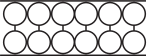
\includegraphics[width=0.2\textwidth]{images/37_3_129r}\\\protect\rule[0cm]{0.5cm}{0cm}\normalsize\textit{[Fig. 1]}
%                        %\caption{Bildbeschreibung}
%                        \end{wrapfigure}
%                        %@ @ @ Dies ist eine Abstandszeile - fuer den Fall, dass mehrere figures hintereinander kommen, ohne dass dazwischen laengerer Text steht. Dies kann zu einer Fahlermeldung fuehren. @ @ @ \\
                \footnotesize mais d'une pression exterieure. \edtext{Comme par exemple si l'on supposeroit, que les corps\protect\index{Sachverzeichnis}{corps} sensibles soyent compos\'{e}es de quantit\'{e} de petits globes en forme de terrelles magnetiques, qui s'attachent comme deux aimants.}{\lemma{}\Afootnote{Comme [...] qui \textit{ (1) }\ se \textit{ (2) }\ se lien \textit{ (3) }\ s'attachent comme deux aimants.  \textit{ erg.} \textit{ L}}} Autrement la separation transversale seroit \edtext{aussi}{\lemma{seroit}\Afootnote{ \textit{ (1) }\ aussi \textit{ (2) }\ autant \textit{ (3) }\ aussi \textit{ L}}} difficile que la directe. Contre le \textso{phenom. 9.} car on a trouu\'{e} que \edtext{les}{\lemma{}\Afootnote{les \textit{ erg.} \textit{ L}}} deux placques glissent ais\'{e}ment l'une sur l'autre, même dans le vuide\protect\index{Sachverzeichnis}{vide}, pendant qu'elles resistent \`{a} la separation perpendiculaire.
                \pend 
                \pstart \footnotesize\textso{Conseq. 4.} Il s'ensuit donc, qu'il reste tousjours quelque matiere dans la cavit\'{e} du Recipient, dont on a tir\'{e} l'air \edtext{sensible}{\lemma{}\Afootnote{sensible \textit{ erg.} \textit{ L}}}, qui puisse exercer cette pression sur les deux corps\protect\index{Sachverzeichnis}{corps} attachez ensemble. \edtext{Contre ceux qui croyent avoir demonstr\'{e} par l\`{a} un Vuide\protect\index{Sachverzeichnis}{vide} veritable}{\lemma{}\Afootnote{Contre [...] Vuide\protect\index{Sachverzeichnis}{vide} veritable \textit{ erg.} \textit{ L}}} je ne dis pas pourtant, qu'il y a des pores dans le verre pour le passage de cette matiere. Car on pourra peut estre expliquer tout cecy par la \edtext{\edlabel{seulestart}seule pression de l'air rarifi\'{e} qui reste dans  le Recipient, laquelle toute petite qu'elle est, est infinie,  quand elle agit contre un rien, ou contre  une place vuide. Au moins le contraire  n'est pas encor demonstr\'{e}.}{\lemma{seule}\xxref{seulestart}{seuleend}\Afootnote{ \textit{ (1) }\ propagation des pressions, qui passent partout. \textso{Conseq. 5.} Il faut aussi que cette pression se fasse par un mouuement ou par un effort \textit{ (2) }\ pression [...] qu'elle  \textbar\ est, \textit{ erg.}\ \textbar\ est [...] demonstr\'{e}. \textso{Conseq. 5.}  \textit{ L}}}%
                     \pend 
                     \pstart\footnotesize \textso{Conseq. 5.} \edlabel{seuleend} On pourroit bien expliquer le \textso{phenomene 9.} o\`{u} l'attachement de deux placques dans le Vuide\protect\index{Sachverzeichnis}{vide} par une Liqueur\protect\index{Sachverzeichnis}{liqueur}, ou matiere subtile\protect\index{Sachverzeichnis}{mati\`{e}re!subtile}, dans laquelle on suppose un mouuement en tous sens, dont les vagues frappent les superficies exterieures des placques. \edtext{\edlabel{carstart}Mais on aura de la peine \`{a} expliquer par l\`{a} le phenomene de la liqueur purg\'{e}e d'air.}{\lemma{placques.}\xxref{carstart}{carend}\Afootnote{ \textit{ (1) }\ Mais outre que cette sorte de mouuement est purement suppos\'{e}e, et semble se d\'{e}truire elle même; \textit{ (2) }\ Mais on aura de la peine \`{a} expliquer par le mouuement d'une  \textit{(a)}\ liqueur\protect\index{Sachverzeichnis}{liqueur|textit} \textit{(b)}\ matiere subtile\protect\index{Sachverzeichnis}{mati\`{e}re!subtile|textit} en tous sens, les phenomenes de la liqueur purg\'{e}e\protect\index{Sachverzeichnis}{liqueur!purg\'{e}e|textit} d'air. Ca \textit{ (3) }\ Mais [...] Car \textit{ L}}}%
                     \pend 
                     \pstart  \footnotesize
                   Car\edlabel{carend} le mouuement de cette matiere subtile\protect\index{Sachverzeichnis}{mati\`{e}re!subtile} continuera, quand même il y aura de l'air engendr\'{e} dans la liqueur\protect\index{Sachverzeichnis}{liqueur}; et comme \edtext{ce mouuement est}{\lemma{comme}\Afootnote{ \textit{ (1) }\ il est \textit{ (2) }\ ce mouuement est \textit{ L}}} capable de presser la liqueur\protect\index{Sachverzeichnis}{liqueur} vers la surface interieure du verre malgr\'{e} sa pesanteur, il sera aussi capable d'empecher, qu'une petite bulle d'air se mette entre deux, et